\documentclass[12pt]{article}

\author{Carter Koehler\\{\small Advisor: Matthew Plumlee}}
\title{Locating Error in Dynamical Systems}
\date{03/19/2022}

\usepackage{amsmath}
\usepackage{amssymb}
\usepackage{graphicx}
\usepackage{float}

%% \usepackage{fullpage}


\newcommand{\cn}{$^{\textit{[citation needed]}}$}
%% \usepackage{}


\begin{document}

\maketitle



\begin{abstract}
  
\end{abstract}


\section{Notation}

\begin{itemize}

\item
  $k$: Number of dimensions of state vector

\item
  $N$: Number of time points

\item
  $t_i$: Time at point $i$

\item
  $\beta$: Parameters of a given model, usually those being estimated.
  
\item
  $x_i^* \in \mathbb{R}^k,\, i=1,\ldots, N$: State vector of the ``true'' model at time $t_i$. 

\item
  $x_i \in \mathbb{R}^k,\, i=1,\ldots, N$: State vector of the approximate model at time $t_i$. 

\item
  $y_i^*$: Diff vector for the exact model, $y_i^* = x_{i+1}^* - x_i^*$
  
\item
  $y_i$: Diff vector for the approximate model, $y_i = x_{i+1} - x_i$

\item
  $f_0: \mathbb{R}^k \to \mathbb{R}^k$: Basic model, which is known in principle.


\item
  $m^*: \mathbb{R}^k \to \mathbb{R}^k$: Unmodelled terms in a system. In principle not known.
  
\item
  $n$: Number of basis functions we search over when looking for unmodelled terms.
  
\item
  $\eta \in \mathbb{R}^n$: Parameters associated with the functions in our search basis.

\end{itemize}



\section{Introduction}

\subsection{Direction}

Dynamical Systems models have been used to great effect in a variety of different fields, and though analysis of these models is well-worn ground, some problems remain when it comes to comparing predictions by the model to real-world data.


First and foremost is the issue of parameter estimation. Though frameworks exist for estimating the constant parameters of a differential equation, such frameworks run into a variety of problems, including$\ldots$


The problem we will focus on primarily is the issue of locating sources of error in dynamical systems. If a proposed model gives us a certain quantity of error, how do we know what causes that error? Is it the result of unmodelled effects in the right-hand sides of our equations? If so, can we learn those effects given some guesses of their shapes? How much error is coming from discretizing the time steps, and can we estimate that and try to account for it when making predictions? And last, how much of the error we see can we attribute to ``true'' noise or measurement error? Many attempts have been made, with more or less success, to address these issues, but few have attempted to look at these problems in a unified way and attempted to tackle the problem of uncertainty in dynamical systems as a single problem.


These are obviously very large problems, and we won't try to solve all of them forever in this limited research span, but we think that approaching them as a unified problem will provide useful ways of thinking as the field progresses.


The dynamical systems we will look at\---and the questions we try to answer\---can take multiple different forms, but the basic problem from which all others descend concerns the general system $$\dot{x}(t) = f(x,t;\beta)$$

Though most of these methods work in the general case, all of the systems we actually look at will have eno direct dependence on $t$, so we will ignore it going forward and just write $f(x;\beta)$.


\section{Background}

\subsection{Parameter Estimation}

The first problem we are interested in is estimating $\beta$. That is, given $f(x;\beta)$ and a set of observations $y_1, \ldots, y_N$, can we find $\beta$ to within a reasonable error margin? Perhaps unsurprisingly, this is a well-worn problem with many different solution methods.

Gelman, et al. (1996) solved a particular instance of this problem, related to pharmacokinetics, using a hierarchical Bayesian approach. They began with a Bayesian prior describing the parameters of their model, under which they numerically solved the dynamical systems and then used the resulting error distributions to update their paramter distributions using fairly standard Monte Carlo methods. One advantage this gave them in their particular case was that it allowed them to jointly construct a population model and individual models by exploiting the hierarchical nature of Bayesian models.\cite{gelman} However, for a general problems their method has a litany of problems, including that there are not always obvious choices of prior, and the computation of posterior is not always tractable.

More recently, the Bayesian approach for parameter estimation has fallen out of favor and been largely replaced by collocation methods, like those used in Ramsay, et al. (2007), which treats the problem as a nested optimization, which considers the solution of the system as a sum of basis functions. They optimize in their outer loop over the parameters, checking for fit against observed values, while their inner loop finds the coefficients of the basis functions which give the optimally-fitting function to the system for a given set of parameters.\cite{ramsay} This generally gives good estimates to the parameters in question, but it gives almost no indication of how good they are.

Even more recently, methods from machine learning have been brought to bear on this problem. Levine and Stuart (2021) use RNNs to solve not only the problem of parameter estimation, but also the issue of discovering model error, which is broadly defined as errors resulting from a misspecified or underspecified model. For example, if one sets $\dot{x} \propto x$, but in reality $\dot{x} \propto x^2$, there is no way to recover the ``real'' model through simple parameter estimation. Their methods are remarkably powerful and show additionally that starting with an educated guess of the true model can cause RNNs to perform much better than they would on their own. However, there are a variety of questions that go unanswered. For example, how much uncertainty can we expect in these estimations in general? And how can we ensure that the parameters we discover, as well as our starting model, are uniquely meaningful, and that we don't just absorb the ``known'' model in our discovered model?


\subsection{Uncertainty Quantification}

In addition to finding the parameters of the dynamical systems we are interested in, we would also like to know the uncertainty associated with our estimates. This is mainly for the purpose of determining when the solution is ``found'' to within a specified tolerance. Techniques exist for determining worst-case error, but in practice the error estimates never reach below desired thresholds, leading to the need for other heuristics to determine when enough data has been collected, among other controlling factors.\cn However, precise knowledge of uncertainty can also used to better estimate the solution and parameters of the system when working under a Bayesian framework, as proposed in Chkrebtii, et al. (2016). However, this naturally requires the use of Bayesian methods, including Markov Chain Monte Carlo methods, which have a variety of problems that can arise, not the least of which that they are not guaranteed to converge, and that it can be difficult to tell when they have converged.

These problems are difficult to avoid, however, when quantifying uncertainty. Most current methods of uncertainty analysis require the use of Bayesian methods of solution, primarily because the posterior distribution of an estimated parameter typically comes packaged with a measure of variance. For example, Cockayne, et al. (2019) lays out a set of reasonable conditions under which the solution to a Dynamical Systems attained using Bayesian methods can give the average-case error\cite{cockayne}.


\section{Current Project}

Of course, solving all of the problems in the field of Numerical Solutions to Dynamical Systems, while something we would like to do, is a bit of a tall ask for a rather limited research period, and we include the above sections mostly to give a sense of the broad direction we would like to go in our research. For the time being, however, we will be content to reproduce some of the results found in the papers listed above, and to provide a limited proof of concept for some of our own methods.

Our work here will follow most closely from Levine and Stuart (2021) and will focus primarily on cases in which the main model\---including parameters\---is known, or at least hypothesized, but misses extra terms in the right-hand side of the system. In particular, if we consider the system describing the evolution of the state $x \in \mathbb{R}^m$ according to the system $$\dot{x} = f(x;\beta, \eta)$$ where we further divide the right-hand side into the known part and the unknown part, say $f^*(x;\beta, \eta) = f_0(x; \beta) + m^*(x; \eta^*)$, where $f_0$ and $\beta$ are assumed known, while $m^*$ and $\eta^*$ are assumed unknown. For the present project, we assume that $m_j^*(x) = \sum_{i=1}^k \eta_{ij} m_i(x)$ is a superposition of known, elementary functions of $x$, scaled by the parameters in question, $\eta^*$, though we expect this to generalize to cases where the form of $m^*$ is more complicated and we have to search over a set of basis functions, such as the spline functions that approximate well any function over the domain in question. Our goal is to learn the values of all the $\eta^*_{ij}$ through observing data generated by the perturbed system. We will write our approximations to the added model as $m(x,\eta)$, where for the current project $m$ can be assumed to be identical to $m^*$, and each $\eta_{ij}$ approximates the true $\eta^*_{ij}$.

We should note here, in order to justify our referring to $m^*$ as a perturbation, that we will assume $||f_0|| \gg ||m^*||$.




\section{Methodology}

We have already laid out several approaches to solving this problem, most of which have been Bayesian. We will take an approach designed to leverage more recent developments in the fields of machine learning and numerical optimization, in particular the \textit{autograd} functionality of \textit{torch}, which allows us to backpropagate error through nearly any operation we can think of.



\subsection{Backpropagation-Based Optimization}

Our main approach to learning the small parameters $\eta_{ij}$ of our model involves fairly straightforward backpropagation. We choose a suitable norm $\|\cdot\|$ and a suitable way to make predictions, the details of both of which are discussed further in (\ref{norms}). Then we let \textit{torch} handle the details of computing the gradients with respect to $\eta$ of each step in the computation of our predictions, which will produce an update for each value of $\eta$. We can also check, for processes that are reasonably approximated by linear functions, that the updates to $\eta$ are reasonable by computing simple finite differences, along the lines of $$\delta\eta_{ij} = \frac{ \| x(\eta + \varepsilon p_{ij}) \| - \| x(\eta - \varepsilon p_{ij}) \| }{2 \varepsilon}$$ Where $p_ij$ is chosen as the such that of its $ij^{th}$ element is $1$ and all others are $0$.



\subsection{Choice of Evaluation Criteria}\label{norms}

For any such backpropagation method to work, we need both a way to evaluate how good our current value of $\eta$ is and, if we need to update it, which directions we should look in. This requires a method of generating predictions and a loss function to evaluate performance. We will look at two choices.

One way of determining predictions and loss is to numerically solve the ODE for the current value of $\eta$ over the entire time domain and take the 2-norm of the difference with the given data, which in our case will be the solution of the system with the known value of $\eta^*$. We will label this $L: \mathbb{R}^{N \times k} \times \mathbb{R}^n \to \mathbb{R}$, defined by $$ L(x^*, \eta) = \| x^* - x_{\eta} \| $$ where $x^*$ solves $\dot{x}=f_0(x)+m^*(x,\eta^*)$ and $x$ solves $\dot{x}=f_0(x)+m(x,\eta)$.

Another choice of evaluation criterion we wish to look into, which has several notable advantages over this method is what we will refer as the Diff Loss. The main idea behind Diff Loss is that, when we solve an entire system, errors in the solution will propagate forward, so that, for $\ell \gg 1$, we expect $\| x*_{\ell} - x_{\ell} \|$ to be dominated by accumulated error from preveious time points. Thus, most of our error would be noise, either the result of discretization error or from earlier $x_i$s.

We propose to fix this by learning over ``diffs'' of $x^*$, which we will write as $y^*$, defined as $y^*_i = x_{i+1} - x_i$. We will compute our predicted values $y_i$ based on $x^*$ by simply computing the right-hand side of the ODEs for our current $\eta$. More precisely, $$y_i = f_0(x^*_i) + m(x^*_i, \eta),\, i=0,\ldots,N-1$$ Then we compute a loss by merely taking the 2-norm over the true diff and the predicted diff, so that we might write $L: \mathbb{R}^{N \times k} \times \mathbb{R}^n \to \mathbb{R}$ as $$L(x^*, \eta) = \| y* - y_{\eta} \|$$




%% \subsection{Other Things that We May Use for Error Quantification}




\section{Sample Problems}

We mostly concern ourselves with two dynamical systems, which we perturb in known ways. We choose these two primarily because Fitzhugh-Nagumo is very well-behaved and should be easy to learn $\eta$ on, whereas Lorenz-63 is likely to be more difficult, due to its high sensitivity to changes in the model.


\subsection{Fitzhugh-Nagumo}

The Fitzhugh-Nagumo equations are defined as follows:

\begin{align*}
  \dot{V} &= c \left(V - \frac{V^3}{3} + R \right)\\
  \dot{R} &= -\frac{1}{c} \left( V - a - b R \right)
\end{align*}

We won't go too deep into the theory of this system. Its specific history and a more complete description of its behavior of it are given in \cite{ramsay}. For our purposes, we will take $a=0.2,\, b=0.2,\, c=3.0$, which produces oscillations in the state vector, where each variable changes between times of steep increase and times of relatively little change, as shown in Figure 1.

\begin{figure}[ht]
  \centering
  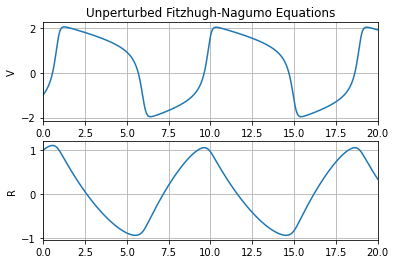
\includegraphics[width=0.7\textwidth]{fn-unperturbed.png}
  \caption{The Fitzhugh-Nagumo Equations with no perturbation.}
\end{figure}



\subsection{Lorenz 63}

The Lorenz-63 System is given as the following:

\begin{align*}
  \dot{x} &= \sigma (y - x)\\
  \dot{y} &= x ( \rho - z ) - y\\
  \dot{z} &= x y - \beta z
\end{align*}

For choices of parameters $\sigma=10,\, \rho=28,\, \beta=\frac{8}{3}$, this produces a chaotic attractor which should look familiar to those inside and outside the mathematical community. The Lorenz attractor is particularly noted because of its sensitivity to small changes in initial conditions and scalar parameters.

\begin{figure}[ht]
  \centering
  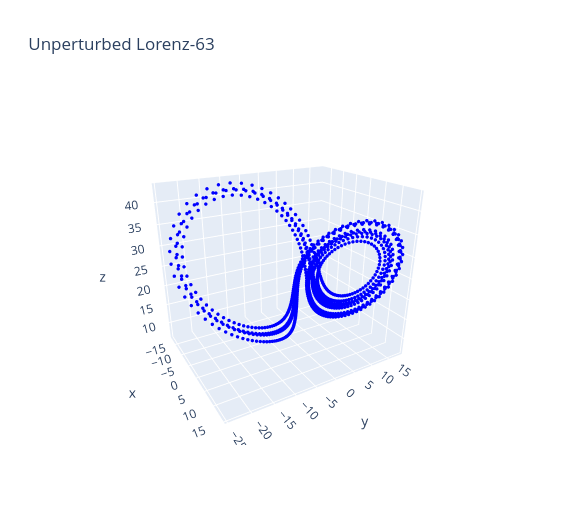
\includegraphics[width=0.9\textwidth]{lorenz-unperturbed.png}
  \caption{The classical Lorenz-63 System}
\end{figure}





\section{Results}


\section{Future Directions}




\bibliographystyle{unsrt}
\nocite{*}
\bibliography{dynsys}


\end{document}
